
\documentclass[10pt,letterpaper]{article}
\usepackage[top=0.85in,left=0.85in,footskip=0.75in]{geometry}
% amsmath and amssymb packages, useful for mathematical formulas and symbols
\usepackage{amsmath,amssymb}
% Use adjustwidth environment to exceed column width (see example table in text)
\usepackage{changepage}
% Use Unicode characters when possible
\usepackage[utf8x]{inputenc}
% textcomp package and marvosym package for additional characters
\usepackage{textcomp,marvosym}
% cite package, to clean up citations in the main text. Do not remove.
\usepackage{cite}
% Use nameref to cite supporting information files (see Supporting Information section for more info)
\usepackage{nameref,hyperref}
% line numbers
%\usepackage[right]{lineno}

\usepackage{natbib}

\usepackage{graphicx}

\usepackage{float}

% color can be used to apply background shading to table cells only
\usepackage[table]{xcolor}

% array package and thick rules for tables
\usepackage{array}

\usepackage{dsfont}


%% END MACROS SECTION

\title{Using Triqler for analyzing Data Independent Aquisition Data}
\author{Patrick Truong \and Matthew The \and Lukas K\"{a}ll}

\begin{document}
%\linenumbers
\maketitle

\begin{abstract}

The estimates of accuracy for differential protein abundance estimates by label-free shotgun proteomics is effected by a wide range of error sources. In an effort to control tyhe errors of the final prediction, we have previously designed an model, Triqler, that combines errors from peptide identification and abundance estimation.
Triqler was designed for handling data from data-dependent acquisition, however, here we demonstrate that the same model can successfully be applied to data-independent acquisition data. Based on a DIA datasets of mixtures of proteomes we observe an improved performance in terms of number of identified differentially abundant proteins compared to other state-of-the-art methods. We also demonstrate that the performance is independent of if peptides are identified with spectral library searching or matching pseudo-spectra with search engines. 
\end{abstract}
  

\section*{Introduction}
Label-free quantification (LFQ) using Data independent acquistion (DIA) mass spectrometry (MS) based proteomics has been shown to be an effective methods for studying the relative concentration of proteins in complex mixtures \cite{venable2004automated}. Compared to Data-dependent axquisition (DDA), DIA allows for a broader dynamical range and more reproducible peptide detection \cite{zhang2020DIA, Lu2021DIAmeter}.

The processing of LFQ data involves several steps, ..., 
 
Triqler is a novel software that uses a probabilitical graphical model for protein quantification and differential expression analysis, essentially eliminating the need for filtering, tresholding and imputational procedures required by many conventional methods. Triqler has been shown to distinguish more proteins for DDA data compared to other DDA protein quantification methods. \cite{The2018Integrated}. 

 
\section*{Materials and methods}
\textbf{Data description}

The data is a DIA dataset used in a previous benchmark of DIA protein quantification benchmarking study [LFQBenchPaper2016]. It is available from the ProteomeXchange Consortium with the dataset identifier PXD002952. The instrumentation used process the data was TTOF6600 system with 32 fixed windows. In the repository the data we use is referred to as the HYE124 hybrid proteome samples. It consists of tryptic peptides with the following ratios: Sample A composed of 65\% w/w, 30\% w/w yeast, and 5\% w/w E. coli proteins. Sample B was composed of 65\% w/w, 15\% w/w yeast and 20\% w/w E. coli proteins. Further details about mass spectrometric instrumentation and data acquisition is available in Navarro et al. [LFQBenchPape2016].     

\textbf{Data preparation and spectral library generation}
The .wiff files are converted to .mzML files in centroided format using msconvert (using windows OS msconver version X.X) with the following options: [check options]. 

Two approaches was used for spectra library generation: DDA acquisition based spectral library generation and Prosit-based spectral library generation using only .fasta file [cite prosit paper]. 

DDA acquisitions of samples from each specie (human, yeast, E. coli) was provided in triplicates for spectral library generation. Uniprot fasta files with one protein seqeunce per gene was concatenated for each specie (UP000005640, UP000000625 and UP000002311, acquired on 2021-06-16).To control for the effect of different protein inference strategies (protein group, parsimony etc.) a modified .fasta file, without shared peptides, was used for database search. The unfiltered fasta files contained 20 590 human proteins, 6 046 yeast proteins and 4 373 E. coli proteins. After filtering the fasta file contained 20 302 proteins (-288 human proteins), 5 848 yeast proteins (198 yeast proteins) and 4 306 E. Coli proteins (-67 E. Coli proteins). Each sequence with length $>$7 amino acids mapping only to one protein. The fasta file contained reverse sequences as decoys for target-decoy analysis. MSFragger with parameters: [check parameters] was used for DDA-search, statistical validation was performed by peptide prophet and protein prophet, and EasyPQP with parameters: [check parameters] was used for spectral library building. OpenSwathDecoyGenerator was used with default setting to generate decoys for the resulting spectral libraries.  

For Prosit-based spectral library generation, the fasta file was converted to prosit input format using encyclopeDIA converter. Prosit\_2020\_intensity\_cid model was used as intensity prediction model and Prosit\_2019\_irt was used as iRT predicition model.  


\textbf{Protein inference problem and reduced database}

In bottom-up proteomics, redundency in the matching of peptides to proteins hits is a challenge \cite{nesvizhskii2005interpretation}. The Parsimony principle reports the minimum set of proteins which include all the observed peptides (Occam's razor principle), thereby resolving shared and ambiguous evidence. This method typically reduces the size of the protein list where peptides could belong to several proteins, as the cost of losing potential protein idenfications. In addition it may also lower the repoducibility of the identified proteins\cite{serang2012recognizing}. While the protein grouping approach bunch together proteins based on different schemas. For example it is possible to group together proteins that map to identical peptides, or when proteins contain overlapping subsets of peptides. The protein groupings are often assigned post peptide identification, which contrary to good statistical practices to formulate the hypothesis before data are observed \cite{serang2012recognizing}. An example of parsimony and protein grouping is shown in \textbf{table 1}. 

\begin{table}[!htbp]
\begin{tabular}{llllllll}
          & Peptides &   &   &   &   & Parsimony reported & Grouping reported \\
          & 1        & 2 & 3 & 4 & 5 &                    &                   \\
Protein A & x        & x &   &   &   & Yes                & Yes               \\
Protein B &          & x & x &   &   & No                 & Yes               \\
Protein C &          &   & x & x &   & Yes                & Yes              	
\end{tabular}
\newline
\textbf{Table 1:} Example of Parsimony reported and protein grouping reported proteins.
\end{table}

In this benchmarking stude we remove proteins with shared peptides. Using different methods for protein inference yields different amount of protein matches given the same amount of observed peptides. Ideally, the number of proteins compared between different protein quantitation methods should be the same when benchmarking. By removing proteins with shared peptides from the FASTA-database the protein inferences procedures will yield the same protein identifications. This should give a fair comparison regardless of protein inference method used in the different protein quantitation pipelines.

\textbf{DIA methods}
Write about why different methods where used.

\textbf{OpenSwath Analysis}
Version (version) of OpenSwath was used. The spectral library generated above is converted to .pqp format using TargetedFileConverter. Data analysis was conducted using OpenSwathWorkflow with parameters (-Scoring:TransitionGroupPicker:background\_subtraction original -Scoring:stop\_report\_after\_feature -1, -min\_upper\_edge\_dist 1, -tr\_irt hroest\_DIA\_iRT.TraML, -extra\_rt\_extraction\_window 100, -min\_rsq 0.95, -min\_coverage 0.6, -Scoring:Scores:use\_dia\_scores true, -rt\_extraction\_window 600, -mz\_extraction\_window 30, -threads 10, -Scoring:DIAScoring:dia\_extraction\_unit ppm). After data extraction the data .osw output was merged using pyprophet merge option and pyprophet was used for statistical validation. Pyprophet export was used without FDR filtering (--max\_global\_protein\_qvalue 1.0, --max\_global\_peptide\_qvalue 1.0, --max\_rs\_peakgroup\_qvalue 1.0, --max\_transition\_pep 1.0) to give a complete list of peptide quantifications for further down-stream analysis.

\textbf{DIAUmpire and DIA-NN analysis}
DIAUmpire signal extraction (SE) was used through Fragpipe GUI (v15.0). Default parameters was set (MS1 PPM: 10, MS2 PPM: 20, Max Missed Scans:1, Mass Defect Filter On, RP max: 25, RF max: 500, Corr Treshold:0, Delta Apex: 0.2, RT Overlap 0.3, Mass Defect Offset 0.1, Isotope Pattern: 0.3, MS1 SN: 1.1, MS2 SN 1.1, Adjust fragment intensity On). MSFragger was used on the resulting .mzML files from DIAUmpire SE with default parameters for Peak Matching (PPM: [-20, 20], Fragment mass tolerance PPM: 20, Calibration and Optimization: Mass Calibration, Parameter optimization, Isotop error: 0/1, Data type: DDA, ), protein digestion (Load rules: stricttrypsin, Enzyme name: stricttrypsin, Cut after: KR, Cleavage: ENZYMATIC, Missed cleavages: 2, Clip N-term M: On, Peptide length 7-50, Peptide mass range: 500-5000, Split database: 1) and Modification (Variable modifications: M, \/[\^, Fixed modification: "all selected"). 

\textbf{EncyclopeDIA and PECAN analysis}
Prosit was used to contruct spectra libraries from the modified fasta files. The fragmentation model used was "Prosit - Model - Fragmentation" and the iRT model "Prosit - Model - iRT" (available from https://figshare.com/projects/Prosit/35582).

...


\textbf{Protein quantification}

\textbf{Variance structure}
(Write why different protein quantification methods and the why triqler should be better in theory.) 

The field of protein quantification is relatively new. Many protein quantification methods have been developed specifically for DDA data. Many of these methods should be generalizable for DIA data. Triqler (probabilistic graphical model), MsStats (linear mixed model) and MSqRob (Ridge Regression) all require homoskedastic varaince. In fig. it is show that the variance-to-mean intensity ratio does not increase for larger means (I COULD TRY TO SHOW THIS WITH QQ PLOT INSTEAD). 

\begin{figure}[htp]
    \centering
    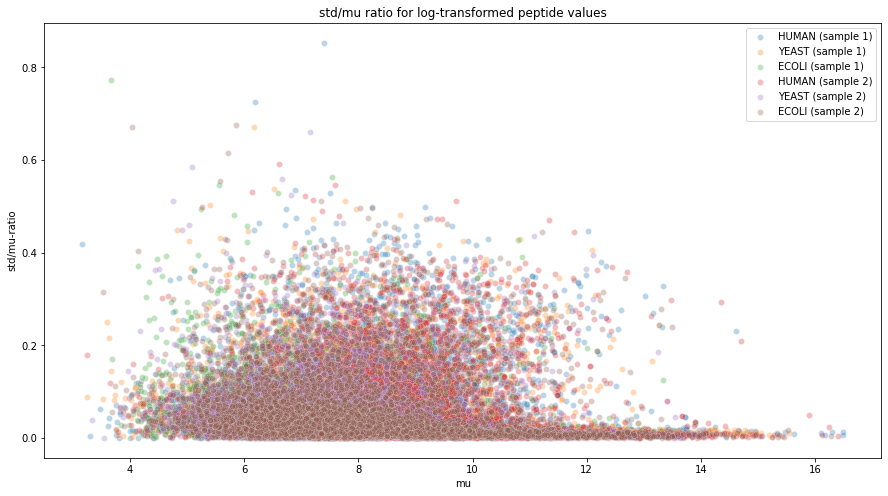
\includegraphics[width=12cm]{../../result/2021-08-13_docs_plots/variance_to_mean_plot.png}
    \caption{mean vs. variance-to-mean ratios. The variance-to-mean ratios stays similar across the means.}
    \label{fig:variance_to_mean_ratio}
\end{figure}

\textbf(Protein quantification tools)


\textbf{Triqler}
Triqler was used with --fold\_change\_eval between 0-2 with 0.04 increments. It computes the two-sided differential probability treshold between the two samples given a fold change evaluation limit. 

\textbf{Top3}
The precursors are filtered by q-value > 1\% and the average of the three largest peptide intensities are taken for each protein. Protein with only one detected peptides (single hit proteins) and proteins detected only in two injections are discarded.

\textbf{MSstat}
 MSstats customizes a linear mixed model to the specific experiment and to each protein \cxite{choi2014msstats}. SWATH2Stats was used to convert the osw output files to MSStats input format. dataProcess function in the MSstats package is used for data pre-processing and quality control of the MS runs of the data into quantitative data for model fitting and group comparison (Default parameters was used [specify default parameters]). quantification function in the MSstats package is applied on the pre-processed data to generate the quantification results for each protein.

\textbf{Msqrobsum}
(Note: write something about difference FDR computation method and conservativeness, and why it does not make sense to compare between processing method, but it is ok to compare between post-processing methods)

Fig. X show the protein quantity distributions with the different species; human (orange), ecoli (blue) and yeast (green) highlighted in different colours. The human distribution apex is not centered at 0 in MsStats and MSqRob, while it is centered for triqler and top3. Likewise the distribution for e.coli and yeast is centered towards the true log2 fold change ratios for triqler and top3, while the apexes are skewed towards 0 for MsStats and MSqRob.    

\begin{figure}[htp]
    \centering
    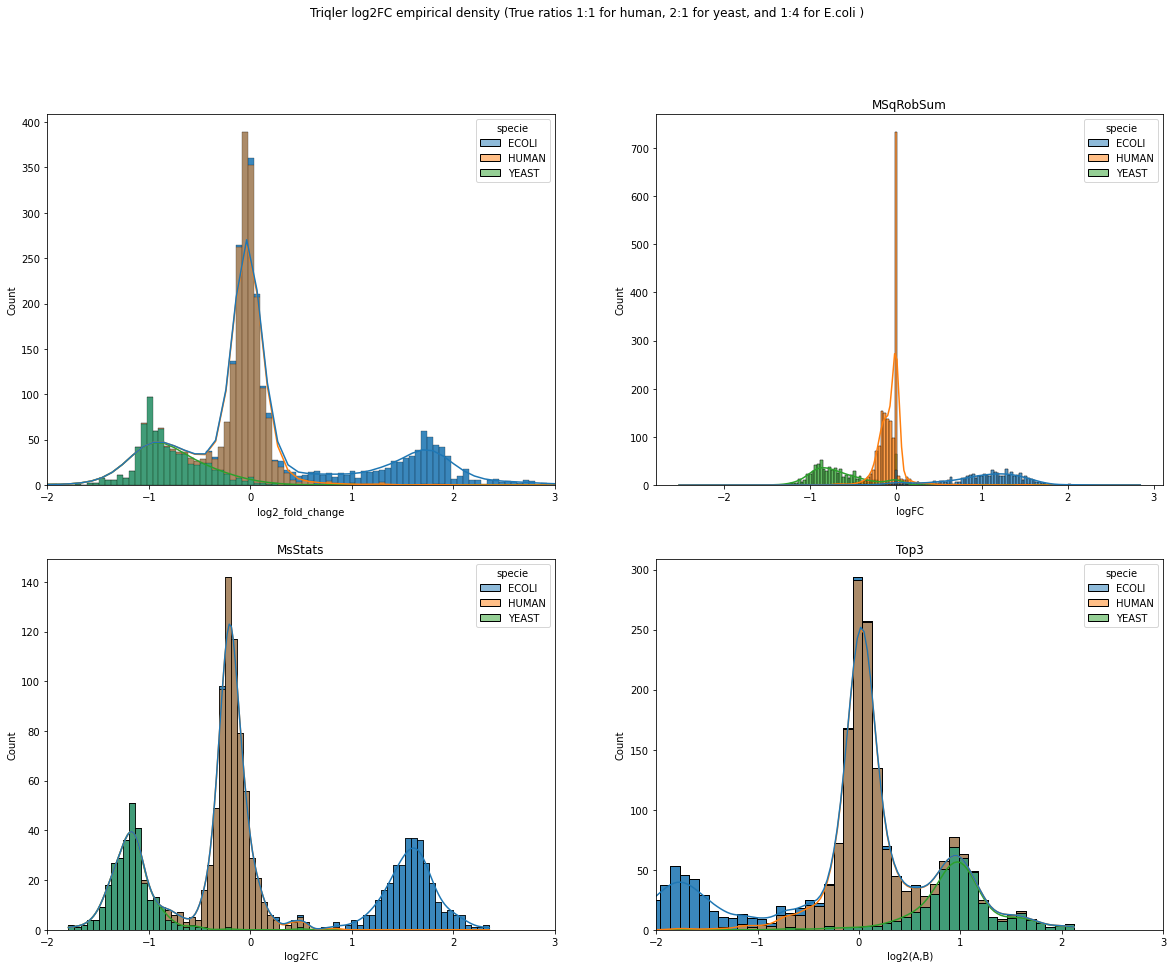
\includegraphics[width=12cm]{../../result/2021-08-13_docs_plots/intensity_plot.png}
    \caption{Protein quantity distributions from Triqler, Top3, MSstats and MSqRobSum at fc = 0.4.}
    \label{fig:intensity_distribution}
\end{figure}


\section*{Results}


\textbf{OpenSwath Analysis}

Fig. Y. show that the number of differentially expressed proteins are significantly higher for Triqler and MSqRobSum at different false discovery rates. MSqRobSum has slightly higher number of differentially expressed proteins than triqler. 

\begin{figure}[H]
    \centering
    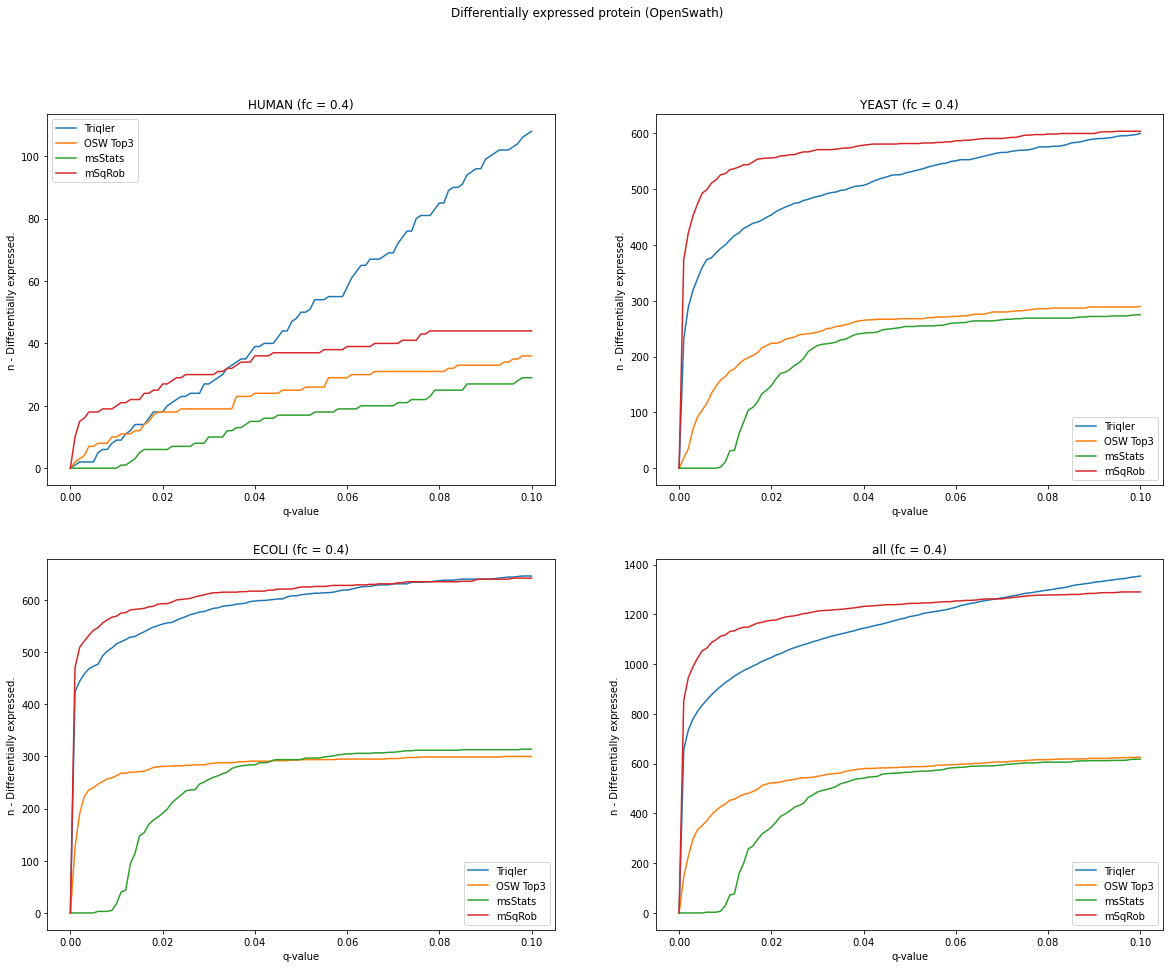
\includegraphics[width=12cm]{../../result/2021-08-13_docs_plots/n_diff_expressed.png}
    \caption{Number of differentially expressed proteins for an OpenSwath analysis with triqler, top3, MsStats and MSqRobSum protein summarization.}
    \label{fig:osw_n_diff_exp}
\end{figure}


However, fig Y shows that the ratio of false positives (human proteins) to number of differentially expressed proteins for a given q-value level is more linear for triqler. At log2FC = 2 all methods are conservative at low q-values. Triqler is better calibrated for low q-values and gets more convervative as the q-value treshold is increased. Top3, MsStats and MSqRob are more conservative at low q-values and gets less convervative as the q-value treshold increases.  

   
\begin{figure}[H]
    \centering
    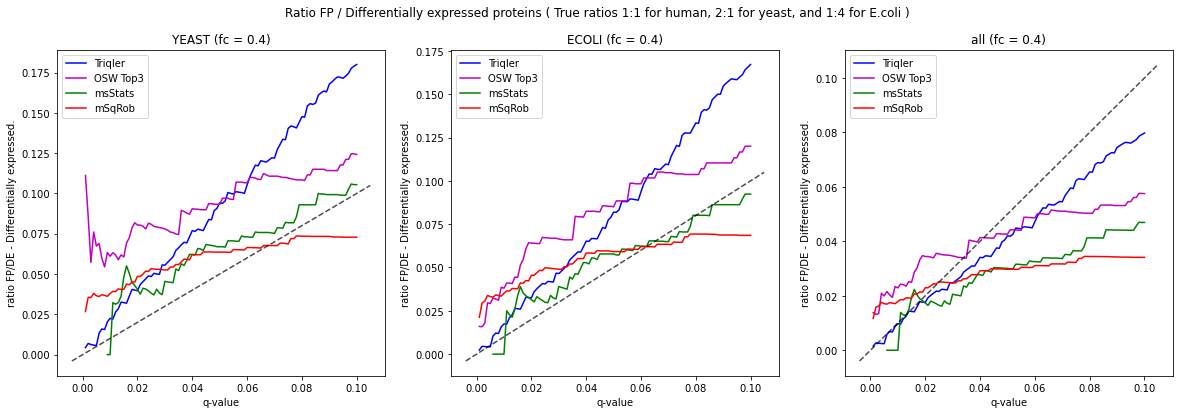
\includegraphics[width=12cm]{../../result/2021-08-13_docs_plots/calibration_plot.png}
    \caption{Q-value (x-axis) and false positive / number differentially expressed protein (y-axis) ratio.}
    \label{fig:osw_n_diff_exp}
\end{figure}


\begin{figure}[H]
    \centering
    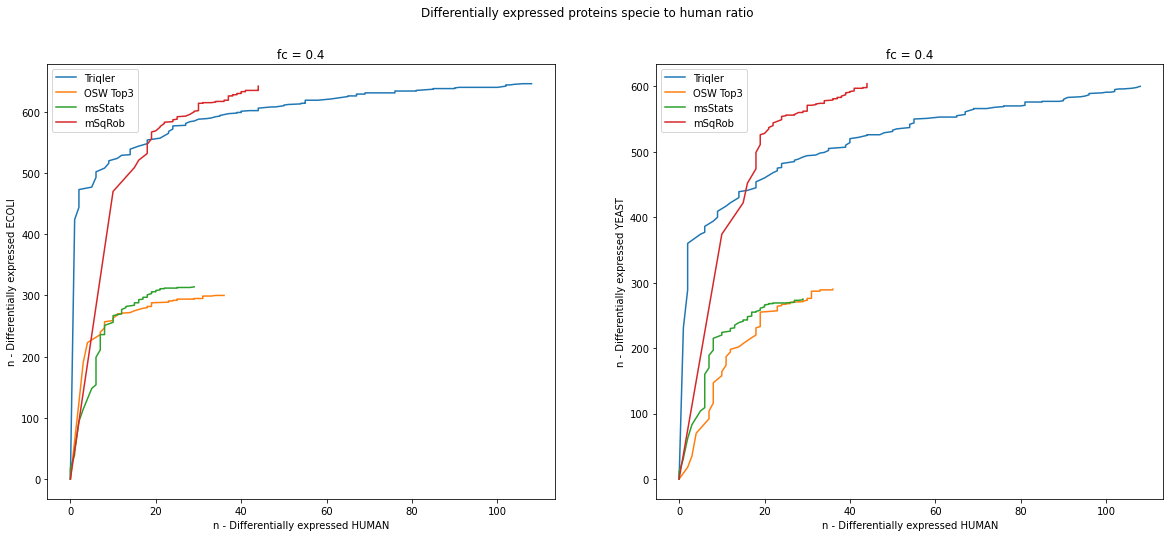
\includegraphics[width=12cm]{../../result/2021-08-13_docs_plots/de_human_vs_de_specie.png}
    \caption{Number of differentially expressed humans (x-axis) and differentially expressed e.coli and yeast (y-axis).}
    \label{fig:osw_n_diff_exp}
\end{figure}



\textbf{DIAUmpire and DIA-NN analysis}

\textbf{EncyclopeDIA and PECAN analysis}


\section*{Discussion}

\section*{Acknowledgements}


\section*{Funding}

This work has been supported by a grant from the Swedish Foundation for Strategic Research (BD15-0043).

\section*{Supporting information}

\bibliographystyle{plain}
%\bibliography{benchmark}
\bibliography{benchmark.bib}
\end{document}

